\documentclass{beamer}

\usepackage[english]{babel}
\usepackage[utf8]{inputenc}
%\usepackage[plainpages=false,pdfpagelabels,unicode]{hyperref}
\usepackage{graphicx}
\usepackage{multirow}
\usepackage{bibentry}

\usetheme{Warsaw}

\begin{document}

\renewcommand{\cite}

\title[Optical properties of dioxides by first principle calculations] % (optional, only for long titles)
{Optical properties of various dioxides by first principle calculations}
\subtitle{The road so far...}
\author{Pavel Ondračka}
\institute
{
	 Faculty of Science, Masaryk University\\
	Brno, Czech Republic
  \and
	CEITEC - Central European Institute of Technology\\
	Brno, Czech Republic
}
\date{17.05.2016}

\maketitle

\begin{frame}
	\frametitle{Outline}
    \tableofcontents
\end{frame}

\section{Motivation}
\begin{frame}
    \frametitle{Motivation}
    \framesubtitle{We want to calculate everything!}
	In theory we could use DFT calculations to:
	\begin{itemize}	
	\item calculate optical properties in broad spectral range (including core electron excitations)
	\item predict optical properties of new materials
	\item better understand underlying processes
	\item help development of new dispersion models
	\end{itemize}
\end{frame}

\section{Introduction}
\subsection{DFT}
\begin{frame}
    \frametitle{DFT introduction}
    \framesubtitle{It shoudl be easy? Right?}

	Hohenberg–Kohn theorems:
	\begin{itemize}
	\item The ground state properties of a many-electron system are uniquely determined by an electron density that depends on only 3 spatial coordinates.
	\item The second theorem defines an energy functional for the system and proves that the correct ground state electron density minimizes this energy functional.
	\end{itemize}
	So we can reduce the many-body problem of $N$ electrons with $3N$ spatial coordinates to 3 spatial coordinates.
\end{frame}

\begin{frame}
    \frametitle{DFT introduction}
    \framesubtitle{Not so easy after all...}

	\begin{itemize}
	\item Born–Oppenheimer approximation.
	\item $\hat{H} = \hat{V} + \hat{T} + \hat{U}$
	\item external potential $\hat{V}$ is system-dependent, kinetic energy $\hat{T}$ and electron-electron interaction energy $\hat{U}$ are not
	\item $E_0 = E[n_0] = <\Psi[n_0] | \hat{H} | \Psi[n_0]> $
	\item $[-\frac{\hbar}{2m} \nabla^2 + V_\mathrm{s} ] \phi_i(\vec{r}) = \epsilon_i \phi_i(\vec{r}) $
	\item $n(\vec{r}) = \sum_i^N | \phi_i(\vec{r}) |^2$
	\item $V_\mathrm{s}(\vec{r}) = V(\vec{r}) + \int{\frac{e^2 n_\mathrm{s}(\vec{r}')}{|\vec{r}-\vec{r}'|d^3r'}} + V_\mathrm{xc}[n_\mathrm{s}(\vec{r})]$
	\item exact form of $V_\mathrm{xc}[n_\mathrm{s}(\vec{r})]$ unknown (LDA, GGA etc.)

	\end{itemize}

\end{frame}

\begin{frame}
    \frametitle{Wien2k}
%    \framesubtitle{}

	\begin{itemize}
	\item All electron full potential fully relativistic DFT code 
	\item LAPW basis
	\item quite cheap licence
	\item included optic package for calculation of optical properties
	\item runs on UNIX and supports heavy parallelisation (k-point, MPI)
	\item in theory the only input needed is the external potential (e.g. unit cell of the material), however due to numerical calculations you need to tweak a LOT of other parameters to reach convergence
	\item periodic boundary condition

	\end{itemize}

\end{frame}

\subsection{Optics}
\begin{frame}
    \frametitle{Selected optical definitions}
    \framesubtitle{What all those letters stand for?}

	There are few terms to describe optical response

	\begin{itemize}
	\item Refractive index $n$ and extinction coefficient $\kappa$, sometimes called complex refractive index $\tilde{n} = n + \mathrm{i} \kappa$
	\item Complex dielectric function $\tilde{\epsilon} = \epsilon_\mathrm{r} + \epsilon_\mathrm{i}$, or for nonisotropic materials dielectric tensor $\hat{\epsilon}$.
	\item $\epsilon_\mathrm{r} = n^2 - \kappa^2 $, $\epsilon_\mathrm{i} = 2 n \kappa$
	\item Absorption (attenuation) coefficient $\alpha = \frac{4 \pi \kappa}{\lambda}$ as known from Beer-Lambert law $I = I_0 \mathrm{e}^{-\alpha x}$  
	\end{itemize} 
	\small
	\begin{equation}	
	\epsilon_\mathrm{i} (E) = 
\left(\frac{eh}{m_\mathrm{e}E} \right)^2 \frac{1}{4 \pi \epsilon_0 \mathrm{B}_0} \sum_{j,k} | p_{j \rightarrow k} |^2
\int_{-\infty}^\infty f_\mathrm{e}(S) \mathcal{N}_j(S) f_\mathrm{h}(S+E) \mathcal{N}_k(S + E)\mathrm{d}S \text{,}
	\end{equation}
	\normalsize
\end{frame}

\begin{frame}
    \frametitle{Selected optical definitions}
    \framesubtitle{No more equations, I promise}

Kramers-Kronig relations:
\begin{equation}
\epsilon_\mathrm{r}(\omega) = 1 + \frac{1}{\pi} \mathcal{P} \int \frac{\epsilon_\mathrm{i}(\xi)}{\xi - \omega} \mathrm{d}\xi \mathrm{,}
\label{KKint}
\end{equation}

So called optical sum rule:
\begin{equation}
\int_0^\infty \epsilon_\mathrm{i} (\omega) \omega \mathrm{d} \omega = \frac{\pi}{2} \omega_\mathrm{p}^2 = \frac{\pi}{2} \frac{e^2 n_\mathrm{e}}{ \epsilon_0 m_\mathrm{e}} \mathrm{,}
\end{equation}

\end{frame}

\subsection{Correct band gap}

\begin{frame}
    \frametitle{Correct band gap}
    \framesubtitle{Its all about the potential}

	DFT is known to underestimate the band gap.

	Possible solutions:
	\begin{itemize}
	\item scissor operator (no additional computational cost)
	\item orbital potential (LDA+U, GGA+U) (same order as LDA or GGA)
	\item mBJ exchange-correlation potential (same order as LDA or GGA)
	\item hybrid potential (expensive)
	\item GW (even more expensive)
	\end{itemize}
\end{frame}

\section{Selected work}
\subsection{HfO$_2$}

\begin{frame}
    \frametitle{Band gap if HfO$_2$ with mBJ}
    \framesubtitle{Looks like a piece of cake}

\begin{table}
\scriptsize \caption{\label{gaps}Overview of calculated band gaps (in eV) compared with experimental data and other \textit{ab initio} calculations.}
\tiny
\setlength{\tabcolsep}{0.5em}
\begin{tabular}{l|cc|ccccc}
 & \multicolumn{2}{c|}{present study} & \multicolumn{3}{c}{literature reports}\\
 & \multicolumn{1}{c|}{mBJ} & PBE & hybrid functionals & GW$_0$ & experiment\\
\hline
m-HfO$_2$ &     5.76 & 4.08 & PBE0: 6.75, HSE06: 5.98 & 5.9 & 5.68 \\
c-HfO$_2$ &     5.88 & 3.77 & SX: 5.6, HSE06: 5.38 & 5.5 & 5.8\\
t-HfO$_2$ &     6.54 & 4.79 & & 6.0 & \\
am-HfO$_2$ & 5.50 & & PBE0: 5.3, 5.94 &  & 5.49--5.72, 5.62, 5.7\\

\end{tabular}
\end{table}

\begin{itemize}
\item The agreement between mBJ and experimntal data is exceptional.
\item What about the dielectric function?
\end{itemize}

\end{frame}

\begin{frame}
    \frametitle{Dielectric function of HfO$_2$ with mBJ}
    \framesubtitle{Using Random Phase Approximation for optics}

\vspace{-0.3cm}
\begin{center}
\includegraphics[width=0.7\linewidth]{figures/all-eps.pdf}
\end{center}

\end{frame}

\begin{frame}
    \frametitle{Dielectric function of HfO$_2$ with mBJ}
    \framesubtitle{Going beyond the RPA}

\begin{itemize}
	\item RPA ignores two particle effects such as excitons
	\item more advanced theory is available - Bethe-Salpether Equation
	\item it contains two particle interaction, however at much greather computational cost
	\item especially the scaling is BRUTAL
	\item $t_{\mathrm{BSE}} = \alpha_\mathrm{scr}(N_\mathrm{v}N_\mathrm{c}N_\mathrm{k})N_\mathrm{q}N_\mathrm{G}^2 + \alpha_\mathrm{ham}(N_\mathrm{v}N_\mathrm{c}N_\mathrm{k})^2N_\mathrm{G}^2 + \alpha_\mathrm{diag}(N_\mathrm{v}N_\mathrm{c}N_\mathrm{k})^3 $
\end{itemize}

\end{frame}

\begin{frame}
    \frametitle{Dielectric function of HfO$_2$ with mBJ}
    \framesubtitle{BSE seems to be a lot better}

    \begin{columns}
	\begin{column}{0.6\textwidth}
	\only<1>{\includegraphics[width=\linewidth]{figures/monoclinic-eps.pdf}}
	\only<2>{\includegraphics[width=\linewidth]{figures/monoclinic-eps2.pdf}}
	\end{column}
	\begin{column}{0.4\textwidth}
	\begin{itemize}
		\item The overall shape is better with BSE but there is approx 1 eV shift
		\item Can we fix this somehow?
		\item Luckily a new mBJ parametrisation is available
	\end{itemize}
	\end{column}
	\end{columns}

\end{frame}

\begin{frame}
    \frametitle{Second look at the band gap values}

\begin{table}
\scriptsize \caption{\label{gaps}Overview of calculated band gaps (in eV) compared with experimental data and other \textit{ab initio} calculations.}
\setlength{\tabcolsep}{0.5em}
\tiny
\begin{tabular}{l|llll|lll}
 & \multicolumn{4}{c|}{present study} & \multicolumn{3}{c}{literature reports}\\
 & \multicolumn{3}{c|}{TB-mBJ} & PBE & hybrid functionals & GW$_0$ & experiment\\
 & orig. & imp. & semi. & & & & \\
\hline
m-HfO$_2$ &     5.76 & 6.01 & 6.54 & 4.08 & PBE0: 6.75, HSE06: 5.98 & 5.9 & 5.68 \\
c-HfO$_2$ &     5.88 & 6.17 & 6.74 & 3.77 & SX: 5.6, HSE06: 5.38 & 5.5 & 5.8\\
t-HfO$_2$ &     6.54 & 6.81 & 7.35 & 4.79 & & 6.0 & \\
am-HfO$_2$ & 5.50 & 5.76 & 6.25 & & PBE0: 5.3, 5.94 &  & 5.49--5.72, 5.62, 5.7\\

\end{tabular}
\end{table}

\begin{itemize}
\item It seems the gaps we get from experiments are misleading.
\item Or at least we still can not get a compatible gap from the theory.
\item Is there a better way?
\end{itemize}

\end{frame}

\begin{frame}
\frametitle{Lets look at the total Density of States (DOS)}

\begin{center}
	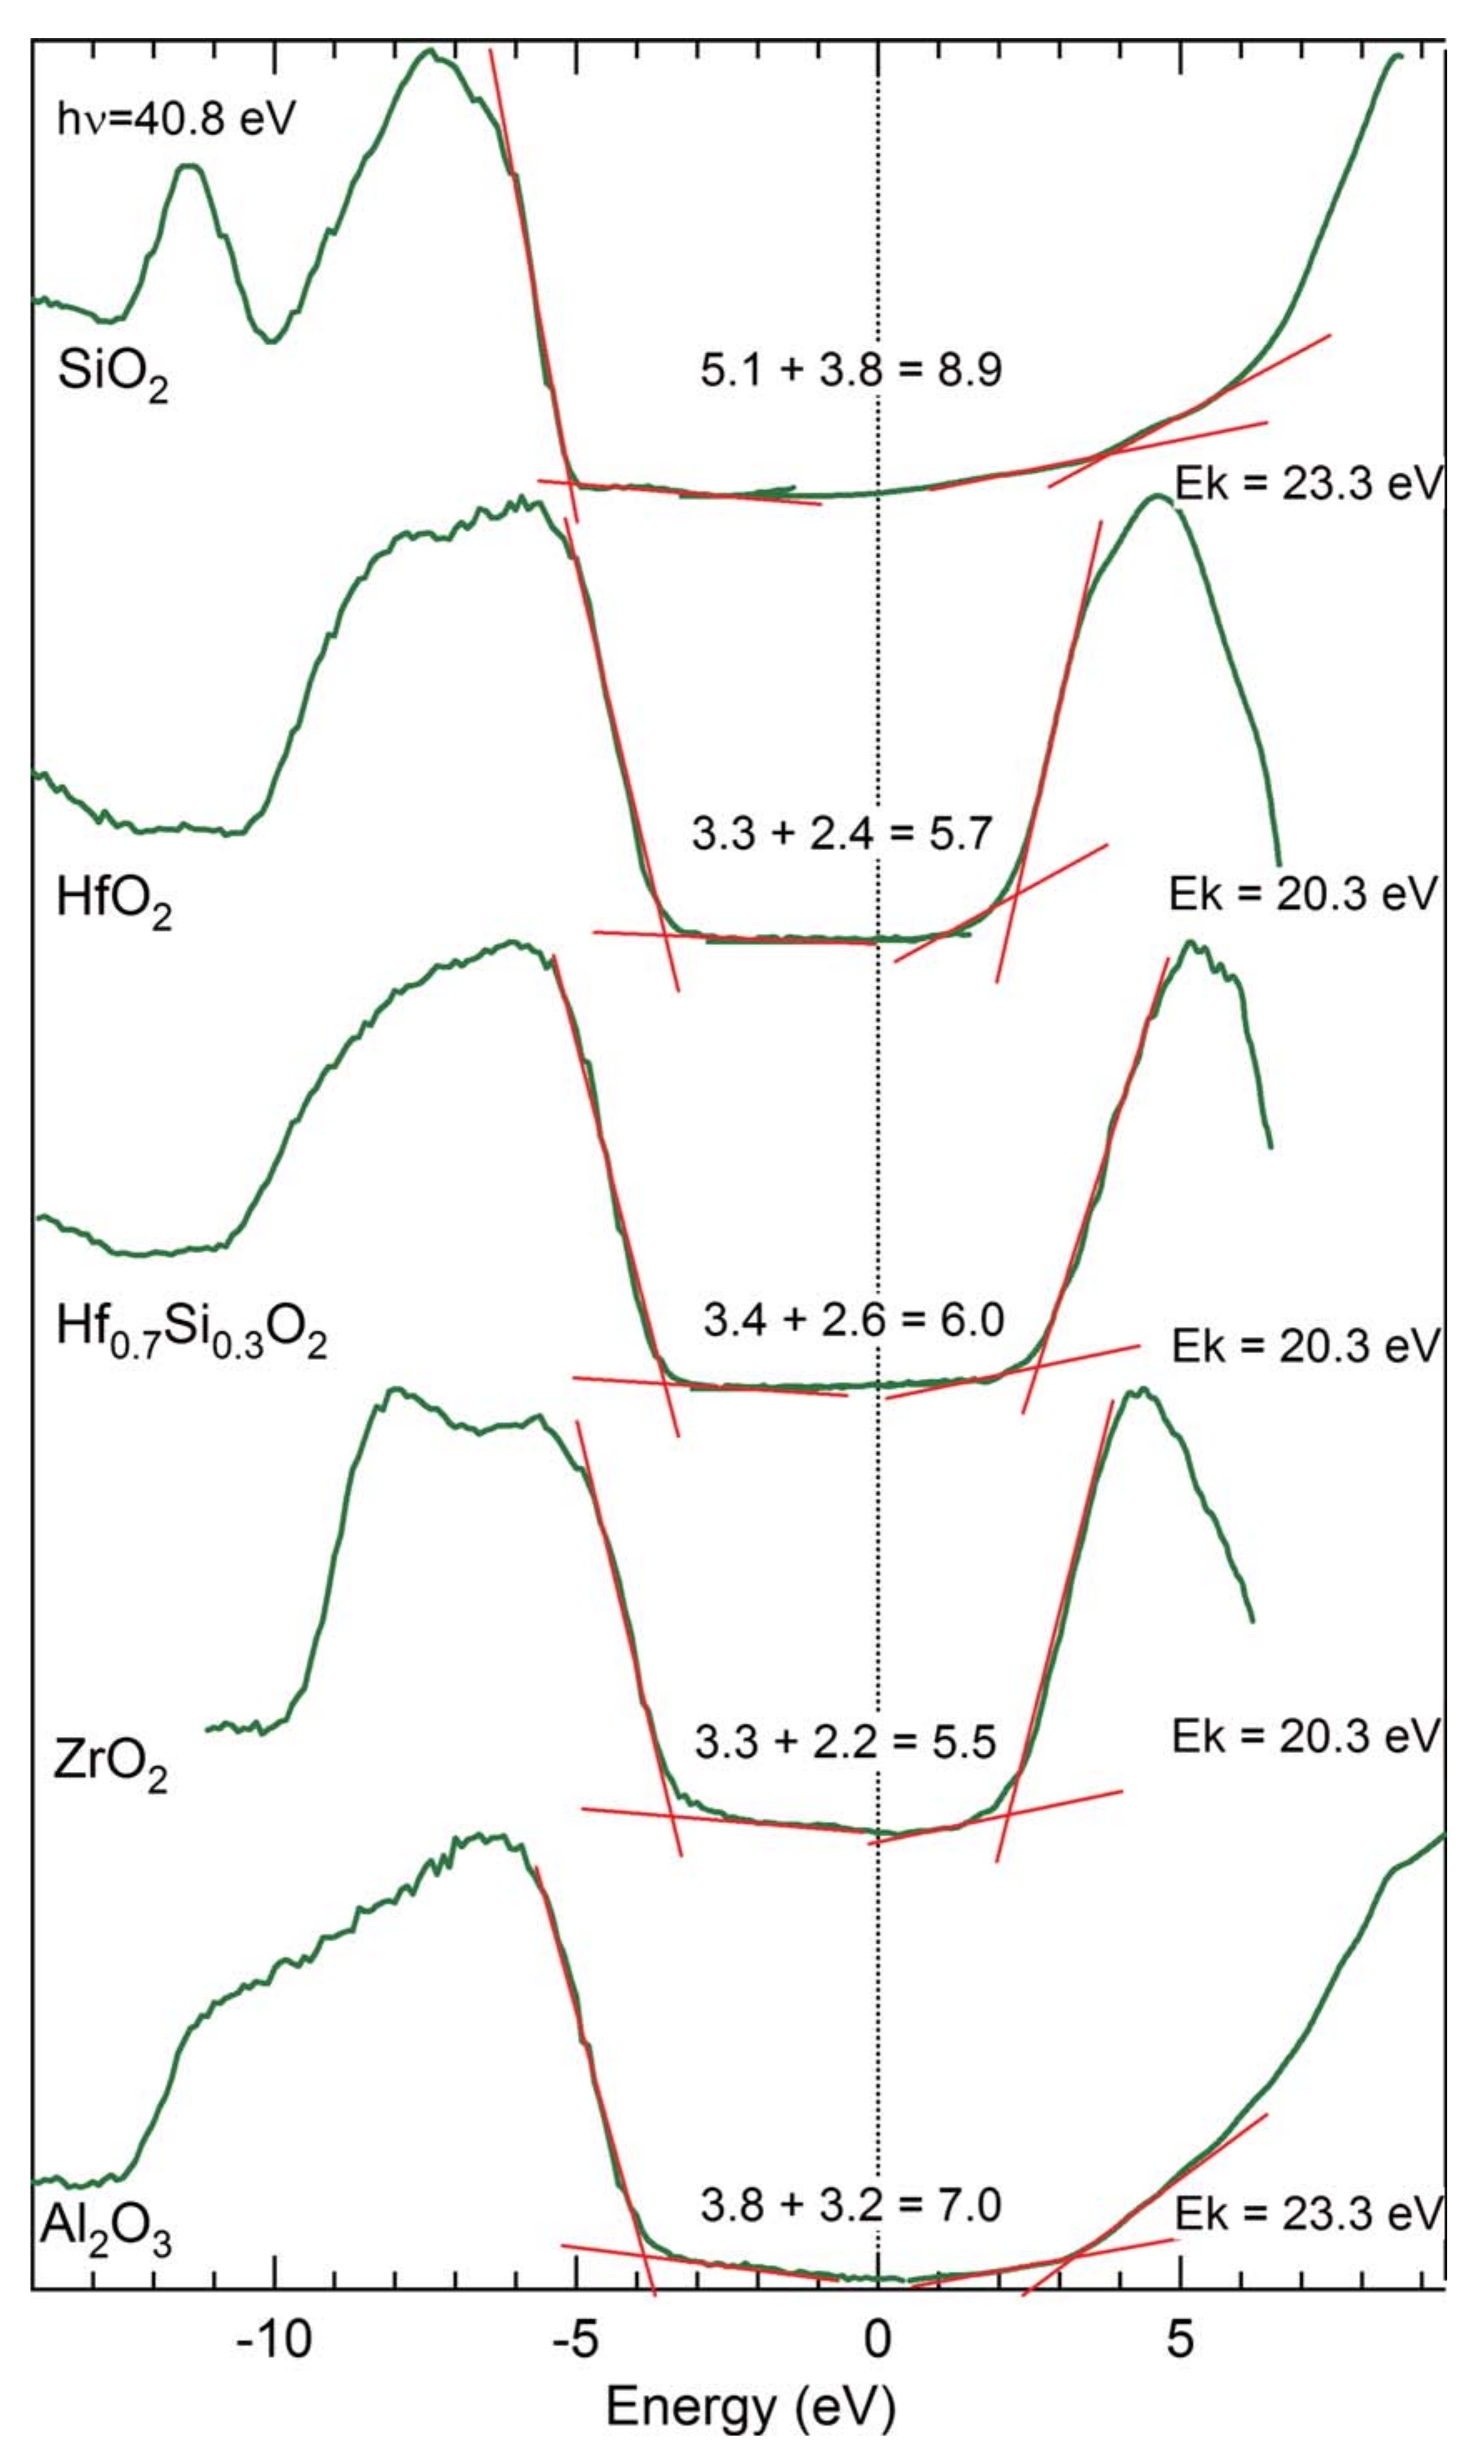
\includegraphics[width=0.7\linewidth]{figures/DOS.pdf}
\end{center}

\begin{itemize}
\item The new mBJ parametrisation (semiconductor) looks much better
\item Directly comparing DOS seems like a good way  
\item But how to get a comparable number for gap?
\end{itemize}

\end{frame}

\begin{frame}
    \frametitle{Experimental band gap of HfO$_2$}
    \framesubtitle{Just to get some ideas how it is done by others}

\vspace{-0.3cm}
\begin{center}
        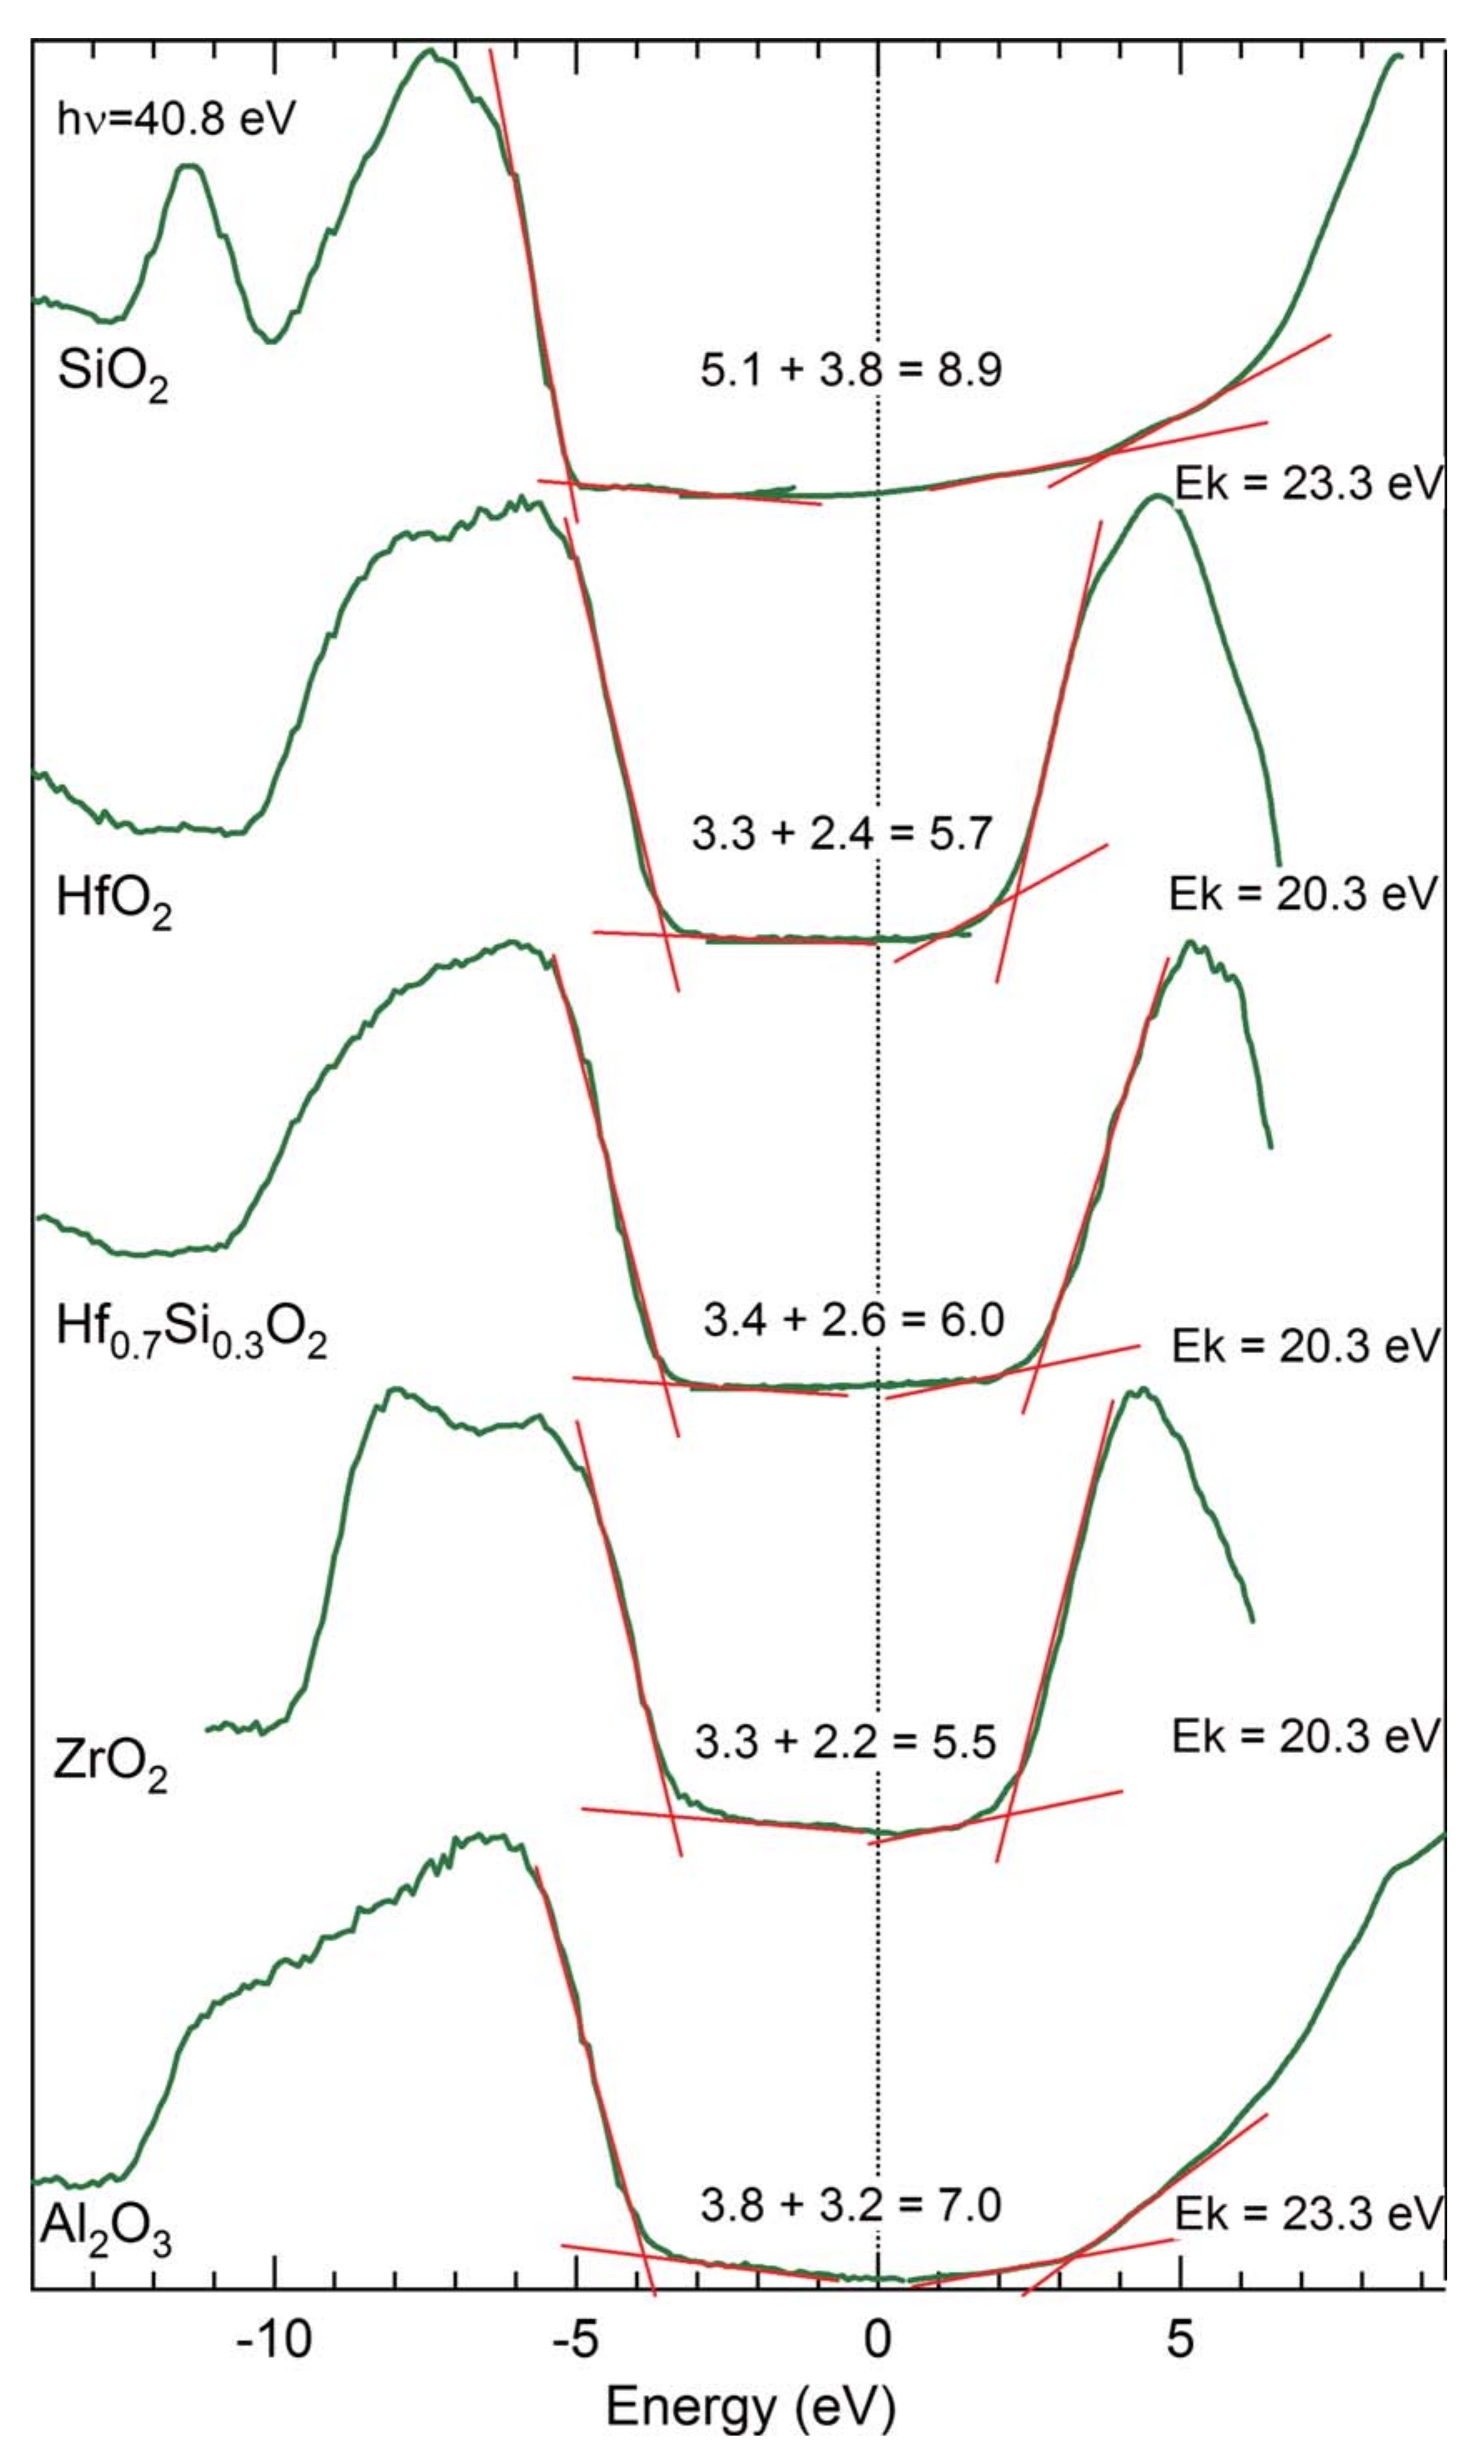
\includegraphics[width=0.38\linewidth]{figures/DOS.png}
\end{center}

\end{frame}

\subsection{Si$_x$Ti$_{1-x}$O$_2$}

\begin{frame}
\frametitle{Si$_x$Ti$_{1-x}$O$_2$}
\begin{itemize}
	\item for TiO$_2$ mBJ and RPA works reasonably well at least in the low energy range
\end{itemize}

\begin{center}
        \includegraphics[width=0.65\linewidth]{figures/compare.pdf}
\end{center}

\end{frame}

\begin{frame}
\frametitle{Si$_x$Ti$_{1-x}$O$_2$}
\begin{itemize}
	\item Comparison with experiment looks very promising expecially for latest amorphous calculations 
	\item Comparison of band gaps is WIP, extreme caution needed to avoid the same pitfalls as in the case of HfO$_2$
\end{itemize}

\begin{center}
        \includegraphics[width=0.65\linewidth]{figures/SiTiO2-n.pdf}
\end{center}

\end{frame}

\begin{frame}
\frametitle{Si$_x$Ti$_{1-x}$O$_2$ XPS}
\begin{itemize}
	\item Last project is the calculation of XPS spectra of Si$_x$Ti$_{1-x}$O$_2$ in order to help with evaluation of experimental data
	\item Main calculations are finished, now working on analysis of data
\end{itemize}

\begin{center}
        \includegraphics[width=0.8\linewidth]{figures/XPS.pdf}
\end{center}

\end{frame}

\begin{frame}
    \frametitle{Conclusion}
    \framesubtitle{Just one more minute, and its finally over}
	\begin{center}Density functional theory\end{center}
	\begin{columns}[c]
    \column{.5\textwidth}
	\begin{itemize}
	\item Can be used to calculate (not only) band gap and optical constants 

	\item Can predict optical constants of new materials

	\item Can shed some light into nature of electronic transitions

	\end{itemize}

    \column{.5\textwidth}

	\begin{itemize}
	\item Extreme caution is needed when choosing the right level of theory or functional for your system 

	\item High computational cost for bigger systems or advanced theory

	\item Your eyes will hurt badly from staring into terminal for long hours.

	\end{itemize}
	\end{columns}
\end{frame}

\begin{frame}
    \frametitle{Questions}
    \framesubtitle{Everything was clear, wasn't it?}

	\begin{center}
	Thank you for your attention.
	\end{center}
	\begin{center}
	Time for questions!
	\end{center}

\end{frame}

\end{document}
